\chapter{Introduction}

The last decade has seen growth in the field of Autonomous
Driving, primarily due to proliferation of graphical processing unit(GPU), and several projects like Google(Waymo) \cite{Waymo},
Berkeley-DeepDrive \cite{Berkeley-DeepDrive}, Apollo \cite{Apollo}, making their datasets
open-source which have made it easier for people to work on these data and achieve better performance gains.

Training a deep neural network(DNN) forms the core of making a car autonomous.
By using supervised learning, reliable results are achieved as it gives greater control
at each stage of training. The data-driven approach collects data in advance and labels it
appropriately. It can be then fed to the DNN using supervised
learning algorithms to train the best model possible.

Ever since the discovery of Alexnet in 2012 \cite{Alexnet2012}, the convolutional neural network(CNN) and
deep learning(DL) are preferred choices to analyse images.  However, it is well known that the camera sensors are susceptible even to a slight change in weather conditions.
Sensors like radar \cite{Radar}, LIDAR \cite{LIDAR}, ultrasonic\cite{ultrasonic}, depth camera
give additional depth information for obstacle detection. These features are then fused
with the camera images and this process is called data fusion.

Even though there are some public data available, it is still not enough to reliably
train a DNN. Then there is  the cost of building an autonomous car. Fortunately, the last
years have seen growth in reliable simulators which
helped massively to collect data to help explore this field of research.
To name a few simulators that are being actively used -- LGSVL \cite{rong2020lgsvl}, Nvidia Drive
\cite{NvidiaSimulator}, Carla \cite{CarlaSimulator}, CarMaker \cite{CarMaker}.
In this thesis, the LGSVL simulator is used.

\begin{figure}[!ht]
    \begin{center}
        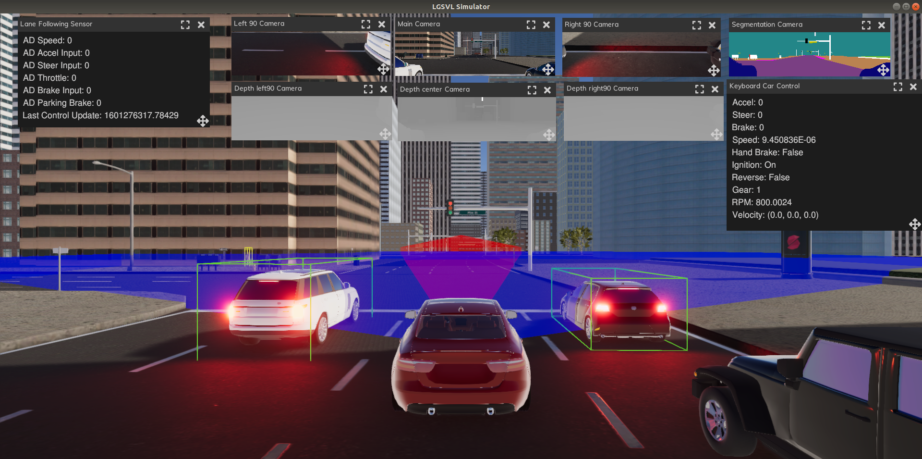
\includegraphics[width=\textwidth]{figures/png/intro/scrot_lgsvl_2.png}
    \end{center}
    \caption{LGSVL\cite{rong2020lgsvl} simulator active with all sensors}
        \label{fig:LGSVL_constellation_sensors}
\end{figure}

The LGSVL simulator allows the use of different sensors with minimal effort. The data
from different sensors are published through websocket. So to capture these data, we
need an interface/protocol which can understand the sent data's message type and enable the
receiving node to store them. However, the data from each sensor arrives at
different rates. Hence it is necessary to collect and synchronise them in the order of their arrival
before storing, so as to not lose their integrity and thereby prevent corrupting the dataset.
Robotic operating system(ROS) \cite{ROS2} and its functionalities fulfil
this purpose. It allows seamless transfer of simulator's data by subscribing to sensor
nodes in the form of topics. Then the subscribing node with the help of ROS libraries, synchronises it as necessary for storage.

So, the data that resembles real-world is stored locally for later analysis and
research.


\section{Motivation}

The motivation for this thesis is to use a simulator, do the required tests, and
determine whether using a simulator does indeed help in perceiving the environment
and accomplishing the goal of driving in the real-world.

One of the major obstacles in autonomous driving is the cost associated with integrating
sensors in addition to manufacturing a vehicle. Representing the environment around the vehicle(ego vehicle) requires information from all in-car sensors.
The resources demanded to make an optimal decision are also a challenge.

The high cost of associated sensors such as LIDAR\cite{mesarticleonLidar}, has put off many smaller research groups from using them
in their work. Simulation allows conducting adequate tests(at a low cost) and quicker
development of algorithms. Simulator provides a safer environment to test and debug these
algorithms.

So with the help of a simulator it is observed how different constellation of sensors work, how different modalities interact with
each other, and what impact these factors have on the overall performance of the deep
neural networks.

Finally, an end-to-end system is implemented which simulates real-world behaviour and gives
results which can then be applied to future research to make it more robust.
%%%%%%%%%%%%%%%
%TODO -
%insert a table 2.1 in page10 showing how different sensor combo work. Use the thesis under
%reference in firefox.
%https://www.researchgate.net/profile/Markus_Weber14/publication/342283221_Autonomous_Driving_Radar_Sensor_Noise_Filtering_and_Multimodal_Sensor_Fusion_for_Object_Detection_with_Artificial_Neural_Networks/links/5eebe41d458515814a6aa417/Autonomous-Driving-Radar-Sensor-Noise-Filtering-and-Multimodal-Sensor-Fusion-for-Object-Detection-with-Artificial-Neural-Networks.pdf
%%%%%%%%%%%%%%%%

\section{Goal}
    The desired goals of this thesis are listed below:

    \begin{enumerate}
    \item Building a basic autonomous driving framework which comprises of the following components:
        \begin{itemize}
        \item ROS - use ROS2 to synchronise the data received from the simulator and its plugin through a
            rosbridge, use functionalities such as slop and cache, to sort the data according to
            their received time in order not to scramble the information. During the evaluation,
            use the same functionalities to send command controls back to the simulator.
        \item Data collection - collect data from the environment.
        \item Training the collected data - preprocess the data to required needs and
            train models using it.
        \item Evaluate the trained models - using ROS connect to simulator, fetch test
            data, repeat the preprocessing steps, use neural network to predict the control commands, and
            feed these outputs to the simulator.
        \item Docker - set up a work environment that is independent of hardware or
            operating system which allows easy running of the commands for data collection
            and evaluation.
        \end{itemize}
    \item Implement an end-to-end neural network architecture which applies state of the
        art deep learning techniques to learn driving by predicting the steering and other
        control commands from image pixels.
    \item Implement and analyse different constellation of sensors with different data
        fusion techniques.
    \end{enumerate}

\section{Related Work}
In 2012, Alexnet \cite{Alexnet2012} used CNNs to do object classification which, then
in Computer Vision became the dominated approach for classification. Both Chen \textit{et
al.} \cite{chen2017} and Bojarski \textit{et al.} \cite{bojarski2016end} extended
\cite{Alexnet2012}'s approach of using CNN and showed that in addition to classification, CNN can
extract features from images. Then they went on to demonstrate through an end-to-end
network(which self-optimises itself based on its inputs), that steering angles can be
predicted to keep the car in the lane of a road.

In a different field, but using CNN, Sergey Levine \textit{et al.}
\cite{GooglePaperonCNNActuation} in 2016 corroborated that it was indeed possible to extract
features with CNN and predict motor control actions in \textit{object picking robots}.

Then, Xu \textit{et al.} \cite{XuGYD16CNNLSTM} in the same year with CNN-LSTM architecture
showed that using the previous ego-motion events helped predict future ego-motion events.
Using CNNs in an end-to-end architecture raised some questions on how it reached its
decisions. So in 2017, both \cite{heatmapsLearning}, \cite{BojarskiCNN1} did visual
analysis after the CNN layers to better understand the module's functionality.
Vehicle control is more than just steering control. For smoother control, acceleration and
braking are necessary besides steering. Both acceleration and deacceleration are dependent on  the user's driving
style, lane speed limit and traffic etc. Yand \textit{et
al.} \cite{E2EMultimodalDiscreteSpeed} used CNN-LSTM architecture and provided the LSTM
with feedback speed to determine the velocity of the ego vehicle.

Besides vehicle control, perceiving the environment is necessary for collision avoidance.
The RGB colour camera sensors don't provide the depth information which is critical for collision avoidance.
Hence, it is essential to fuse other sensors with diverse modalities with RGB to predict an optimal output.
Liu \textit{et al.} \cite{liu2018learn} provided rules in fusing data. They said that it was
essential to pick out only vital information and discard other noisy data.
They also described the techniques involved in data fusion -- early/late
fusion, hybrid fusion, model ensemble and joint training. Park \textit{et
al.} \cite{ParkHBB16} gave us methods to enhance the features by using feature amplification
or multiplicative fusion. Zhou \textit{et al.} \cite{ZhouSideChannel} detailed how fusing
data into CNN affects the overall performance.

Even though the fused dataset gives a performance boost, it performs worse
compared to individual modality. The combined fused model overfits more
than its counterparts. The fundamental drawback of
\textit{gradient descent} in backpropagation causes the networks to overfit. This paper \cite{wang2020makes} introduced a technique
called \textit{gradient blending} to counteract this problem.

Xiao \textit{et al.}\cite{XiaoCodevillaMultimodalE2E} applied all the fusion techniques
mentioned above with an imitation based end-to-end network\cite{codevilla2017endtoend}.
They concluded that RGB images with depth information(obtained through a different modality)
could indeed result in better performing end-to-end network model.

\section{Contribution}
For supervised learning task, it is essential to collect data and label them. LGSVL, ROS provide an excellent platform to carry out this work.

So with their help, it was possible to acheive
\begin{enumerate}
    \item For the first time implementation of a basic autonomous driving framework based on ROS and LGSVL.
    \item An implementation of an end-to-end training neural network with LGSVL.
    \item Fusing of data with different sensor in different constellations with LGSVL.
\end{enumerate}



